%!TEX root = depicto-top.tex
%%%%%%%%%%%%%%%%%%%%%%%%%%%%%%%%%%%%%%%%%%%%%%%%%%%%%%%%%%%%%%%%%%%%%%%%%%%%%%
%% Conclusion, evaluation, and more
%%%%%%%%%%%%%%%%%%%%%%%%%%%%%%%%%%%%%%%%%%%%%%%%%%%%%%%%%%%%%%%%%%%%%%%%%%%%%%

\chapter{Winding down}
\label{chap:Conclusion}

\section{Progress so far}
\label{sec:conc:progress}

As of May 2016, the basic three-part architecture of the \depicto\ system is in
place and all module-specific extensions (described in \cref{chap:pipeline1}
and \cref{chap:pipelineii}) are in working order (insofar as their experimental
status permits). This means that the system as a whole is able to take a string
of \sclera\ symbol identifiers as input, parse this string for its semantic
structure, modify, or `transfer', the resulting `\mrs' so as to accommodate a
given target language (in this case: Dutch), and, finally, as demonstrated in
\cref{subs:generation}, use this \mrs\ as the basis for generating one or more
grammatical sentences as output.

Of course, only those input strings are accepted which are well-formed with
respect to the constraint-based model of \sclera\ used by the analysis module
(\cref{chap:pipeline1}). Starting from a (purely hypothetical) sketch grammar
of \sclera\ (\cref{sub:sclerastrings}), this model treats \sclera\ as a simple
SVO language that is unique in the fact that it has `invisible' determiners
(\cref{sub:MissingDeterminers}), complex pictographs corresponding to phrasal
constituents of varying saturation (\cref{subs:cs:complex-pictos}), and
`particles' which actively modify the illocutionary force
(\cref{subs:cs:interrogative}) or temporal orientation
(\cref{subs:cs:temp-disambig}) of a \sclera\ utterance. Currently, the model
covers 30 \sclera\ symbols (see Appendix~\ref{app:sclera-lexicon}), each of
which has an equivalent in the next two stages in the processing chain, and
accepts root structures (i.e., typed feature structures that can serve as the
start symbol for parsing) that correspond to a single clause, although
independent noun phrases and various elliptical structures, including discourse
markers, will soon be supported.

Moving on to the other two modules in the system (\cref{chap:pipelineii}), we
first saw how a simple semantic (\mrs-based) transfer grammar for the language
pair \sclera-Dutch is set up (\cref{sec:Semantictransfer}). In the actual
course of development, this step formed something of a milestone, offering
welcome reassurance that the grammar of \sclera\ (\depicto's main contribution)
could indeed stand independently of the rest of the pipeline, amenable to
`co-operation' with other third-party grammars by virtue of an additional
transfer grammar. Since (to the best of my knowledge) the practicalities of
setting up a transfer grammar are not documented in any great detail anywhere,
special attention is paid to the process (\cref{sub:sclera-dutch}) so that this
section may additionally serve as a resource in the future. Finally, for the
last module, a simple grammar of Dutch is developed (\cref{sec:generation})
which, in addition to its basic feature geometry, phrase structure rules, and
lexicon, features two temporary loci of experimentation involving determiners
(\cref{subs:dutch:determiners}) and synonymy (\cref{subs:dutch:synonymy}), the
former eventually to be relocated to another stage of the pipeline so as to
maintain the target language grammar's independence. As discussed in
\cref{subs:generation}, the current version of the \depicto\ system does not
discriminate among the various translation hypotheses produced by the
generation module. As a result, it is still some way away from being ready for
use in real-world (in this case: AAC) applications.

%-----------------------------------------------------------------------------

\section{Evaluation}

In describing the development of \depicto's individual modules,
\cref{chap:pipeline1} and \cref{chap:pipelineii} also provide critical
reflection on the appropriateness of the design decisions taken, particularly
when the proposed solution has the potential of posing a limitation to the
module currently under development. This section takes up a similarly critical
tone, but does so from a holistic standpoint, considering the system not in
terms of its component parts, but as a whole. In \cref{subconc:eval:main}, the
system is evaluated with respect to its ability to produce quality output
(`precision'), its coverage over possible input strings, and its overall
performance in terms of speed. Because \depicto\ is still in an early stage of
development, its lexicon of \sclera\ still relatively minimalistic and its
output unfiltered, metric-based methods for evaluating the system are not
appropriate. Instead, the evaluation process is guided by simple intuition,
i.e., human judgement. In \cref{conc:eval:dep-v-p2t}, the \depicto\ system is
pitted against the \emph{Picto2Text} system developed by
\citet{sevens2015natural} (introduced in \cref{sub:picto2text}). This (largely
playful) comparison serves to illustrate both the strengths and limitations of
\depicto's rule-based architecture in contrast to the (at heart) statistical
approach taken by \emph{Picto2Text}. The results are largely in keeping with
the traditional trade-offs between Rule-Based Machine Translation (RBMT)
systems and Statistical Machine Translation (SMT) systems, but instructive
nevertheless.

\subsection{Precision, coverage \& performance}
\label{subconc:eval:main}

\subsubsection{Precision}
% \label{subs:subsubsection label}

Semantically, syntactically, morphologically, and -- in certain respects --
lexically, the \depicto\ pipeline can be said to produce natural language
translations of very high quality. As demonstrated in \cref{subs:generation},
these are composed of semantically relevant lexical items, which are arranged
in appropriate order and inflected in accordance with agreement or case
requirements, and, more important, consistently correspond to the full set of
all possible readings of the input \sclera\ string, which, as we saw earlier,
the pipeline is able to narrow down if markers of, e.g., mood or tense are
present on the input.

Orthographically, output strings are of adequate quality: spelling is not an
issue, and the first character of output strings is automatically capitalized.
However, the absence of a theory of punctuation in the grammar of Dutch used
here for generation means that the conventions of the target language's
orthographic system are only partially respected. Slightly less trivial (for
the present purposes, at least) is that, while the target language grammar can
be fitted out for synonymy (see \cref{subs:dutch:synonymy}), it currently
cannot account for how different synonyms enter into different collocation
patterns, which results in some target language strings sounding oddly
unidiomatic.

Similarly, on a pragmatic level, not all strings produced by \depicto\ seem as
felicitous as the next, yet as far as the target grammar is concerned they are
all equal. Idiomaticity and pragmatics are common sources of difficulty in
rule-based translation systems \citep{chan2014routledge}, and for the coverage
of either phenomena the pipeline is largely at the mercy of the machinery
provided by the target grammar, which, as explained, could in principle be any
\delphin\ or \mrs-compatible grammar. For the time being, therefore, we can
only put this down as a limitation, although, given the `deep', i.e., semantic,
approach of the \depicto\ system (or indeed, all \logon-based MT systems),
there is room to imagine a grammar in which, if not a system of pragmatics, a
system of collocation is worked out.

Of course, the most obvious limitation as regards the quality of the \depicto\
system's output is that there is simply too much of it: it is an unfiltered,
unsorted list rather than a single translation. One could argue that this is a
feature of the system, in which case the output should be handled by either an
entirely different, possibly third-party, tool or an additional module. In any
case, until a solution is found, \depicto\ does not amount to a true
translation tool in the sense that users are not required to be familiar with
\emph{both} the source and the target languages in order to use it
successfully. We will briefly look at two possible solutions in
\cref{conc:futurework}.

\subsubsection{Coverage}

The \depicto\ system's coverage, i.e., the set of input strings which can be
parsed, transferred, and generated from, is primarily determined by the model
of \sclera\ used by the analysis module (\cref{sec:mini-sclera}), although, of
course, that is assuming that the \sclera\ grammar has equivalents in the
grammars used by the transfer and generation modules, as is the case in the
version of the \depicto\ system developed here.

Currently, the coverage of the
\depicto\ pipeline is limited in (at least) three ways by the grammar of
\sclera.

In the first  place, its lexicon covers only 30 of the (in total) 13,000
symbols comprised by the \sclera\ set. The main reason for this limitation is
that the lexicon, which has been crafted by hand, is costly to extend,
especially since each new addition to the grammar of \sclera\ requires
corresponding additions to the transfer grammar and, in this particular case,
to the target grammar as well (since the grammar of Dutch is developed `in
house'). Because \sclera\ is a closed symbol set, however, the lexical coverage
of the grammar can in theory be made complete, and large parts of this
objective could be realized fairly inexpensively once the lexical modelling
process becomes automated.

In the second place, the grammar of \sclera\ is specified for a fairly strict
set of syntagmatic restrictions which stem from its origins as a
Subject-Verb-Object grammar. As a result, even if the lexicon is extended to
include all \sclera\ symbols, so that any symbol is covered by the grammar, the
analysis module fails to parse the input if it does not adhere to SVO ordering,
which, in this case, has side-effects for adjective-noun and
verb-adverb/adjunct ordering. Given that the \depicto\ system is primarily
designed for users suffering from aphasia, dysphasia, or otherwise exhibiting
agrammatism, this restriction is -- for want of a better word -- nothing short
of silly. At the same time, however, because \sclera\ does not have a case
marking system (which, again, would run counter to the requirements of the
target audience, anyway), total freedom of word order would open the door to
syntactic ambiguity: `dog' in the utterance `dog see bus' could be parsed
either as the subject of the verb or as the object of the verb, and both parses
would be equally valid. Needless to say, this could lead to some fairly serious
confusion in interpersonal communication, as, for example, with `I hate you'
versus `You hate me', which, communicatively, are clearly two very different
beasts. Eventually, a compromise will have to be devised between the usability
of the pipeline for the target audience and the risk of potentially serious
confusion. Pending an adequate solution, the main SVO word order restriction is
maintained, but noun-adjective and verb-adverb order restrictions are soon to
be relaxed.

The third way in which the coverage of the \depicto\ system is constrained by
the grammar of \sclera\ falls into two parts. First, the grammar only accepts
complete clauses or noun phrases as the start symbol for parsing. To support a
more fragmentary style of communication, this restriction will eventually be
dropped, so that \emph{any} phrase or lexical item can be parsed, the effect of
which will be that the analysis module never blocks, i.e., returns an empty
parse. Of course, whether the result of this more permissive style of parsing
can be used for generation will ultimately depend on the start symbol
constraints of the target language grammar. Second, the current grammar is
designed to model discrete utterances, not discourse. When dealing with clausal
input (as in most of the examples in this thesis), it requires the input to be
a single, well-demarcated clause, which, in practice, means that multiple
clauses equals multiple calls to the pipeline. It is common form for simple
constraint-based grammars to focus on parsing individual sentences rather than
stretches of text/discourse; however, in the context of machine translation,
this restriction implies the assumption that one is either translating from
some source text that can be pre-processed into individual clauses (on the
basis of, say, punctuation) or that users have the ability to identify and
enter clauses individually. Since the translation system is intended for
real-time use and punctuation symbols (which are not popular among target users
anyway) have been repurposed (e.g., the question mark symbol in
\cref{subs:cs:interrogative}), the first option is not relevant. Nor is the
second: it stands to reason that if a user is able to identify a discrete
clause correctly, his/her use for the \depicto\ pipeline might be limited.
Given the invalidity of this assumption, the grammar of \sclera\ should
eventually be extended to cover larger stretches of discourse. (Though not
documented anywhere, the ERG \citep{flickinger2014towards} already appears to
do this for English, so a solution to this last restriction might be relatively
easy to implement.)

\subsubsection{Performance}

Whether or not the input string falls within the coverage of the system,
however, the pipeline itself consistently achieves fast processing times.
Initial (and largely informal) tests performed on an Apple Macbook Pro with a
2.6 GHz Intel Core i5 processor and 8 GB of memory suggest that, when passed an
`ill-formed' \sclera\ string or when the target grammar fails to generate, the
pipeline blocks within 10ms to 20ms. When all stages of the pipeline execute
successfully, total processing times tend to range from 20ms to just under
100ms, the bulk of which is spent on generation. The more results the
generation module can produce, the more time is required. Thus, an artificially
complex (yet well-formed and thus plausible) input string such as \texttt{happy
dog give happy girl happy kiss yesterday question}, which corresponds to a
staggering 768 (!) translationally equivalent Dutch sentences, takes an average
of 250ms longer to process. Using this string, \cref{ex:conc:eval:time}
illustrates how these times have been collected. The shell script in this
example is identical to that used to test the pipeline (see Appendix
\ref{app:settingupdepicto}), except that (ignoring the first line) it is
prefixed by the UNIX \texttt{time} utility, which measures the total time taken
for a command or series of commands to execute. Of the the three times measured
by this utility (i.e., \texttt{real}, \texttt{user}, and \texttt{system}), all
data points are based on the value of the \texttt{real} measurement, which
tends to be the least charitable.

\begin{exe}
    \ex
    \label{ex:conc:eval:time}
    {\small
    \begin{verbatim}
  cd PATH/TO/ACE/BINARY/IN/REPOSITORY/DIRECTORY
  time echo "happy dog give happy girl happy kiss yesterday question" |
# ^^^                   ^^^                       ^
# UNIX time utility    string to be parsed       Pipe
      ./ace_osx -g ../mini-sclera.dat |
#                ^^^^^^^^             ^
#             Analysis module        Pipe
      ./ace_osx -g ../transfer-nl.dat |
#                ^^^^^^^^             ^
#          Transfer module           Pipe
      ./ace_osx -g ../mini-dutch.dat -e
#                ^^^^^^^^             ^
#         Generation module          -e flag sets ACE to generate
    \end{verbatim}
    }
\end{exe}

While generation is certainly the most costly stage in the the pipeline, the
\ace\ processor (to which, needless to say, \depicto's processing times owe a
great debt) provides several optimizations, some by default, others optionally,
that speed the process up. For example, when enabled, the
\texttt{index-accessibility-filtering} optimization reduces total processing
times by an average of 30\%. This is already reflected in the measurements
reported above. Of course, no evaluation of performance is truly complete
without some comparison to existing benchmarks. Unfortunately, I am not
adequately familiar with these at present. For now, therefore, it will have to
suffice to note that, when passed `well-formed' input, the \depicto\ pipeline
is capable of producing (if necessary) a \emph{lot} of high quality output in a
period of time which is more or less experienced as an instant, but the
question of whether this `instant' is more instant than the benchmark speeds of
other (kinds of) translation systems is left blank for now.

\subsection{Comparing the \depicto\ and \emph{Picto2Text} systems}
\label{conc:eval:dep-v-p2t}

Let us now take a quick look at how \depicto\ fares against a similarly
purposed translation system that takes a statistical rather than rule-based
approach. A suitable candidate for this purpose is the promising
\emph{Picto2Text} system developed by \citet{sevens2015natural} at the
KULeuven. As explained in \cref{sub:picto2text}, the current version of the
system draws on a trigram language model of the target language (plus Viterbi
decoding) to select the most likely surface form permutations of (reverse
lemmatized) word tokens derived from those WordNet synonym sets which are
associated with selected pictographs. This approach has the advantage of
increasing the coverage of the translation system at a relatively low cost. At
the same time, however, the quality of the output is only as good as the
three-item horizon of the trigram model can account for, and the model, in
turn, is only as good as the corpus upon which it has been trained. So while
\emph{Picto2Text}'s coverage (or \emph{recall}) is comparatively high, its
precision is prone to ceiling effects and its output less easy to predict. This
situation is of course the inverse of the \depicto\ system, where coverage is
low (and relatively expensive to extend), but precision is high and entirely
predictable based on the constraints of the grammar model. The effect of these
opposing traits can be observed when both systems are passed the same input
string. (All interactions with \emph{Picto2Text} happen through the online demo
available at
\href{http://picto.ccl.kuleuven.be/DemoP2T.html}{\texttt{picto.ccl.kuleuven.be/DemoP2T.html}}.
Note that this demo may not represent the most up-to-date version of the
\emph{Picto2Text} system.)

Consider the output of translation by each system for the (by now much-loved)
\sclera\ string `dog see bus', as listed in \cref{ex:conc:dvp1:trans}. (Notice
that this string, like most that follow, is already known to fall within
\depicto's coverage, which does bias the comparison to an extent; I will make
up for this toward the end.) As expected, \depicto's output comprises multiple
translation hypotheses, three of which are shown. \emph{Picto2Text} outputs
only the most likely translation hypothesis, which in this case is the (100\%
grammatical) Dutch sentence \emph{De hond ziet een bus} (`The dog sees a bus').

\begin{exe}
    \ex \label{ex:conc:dvp1:trans} Translating `dog see bus' into Dutch: \\\\
     {
\includegraphics[width=1.5cm]{sclera/hond1}\hspace{0.5cm}}
     {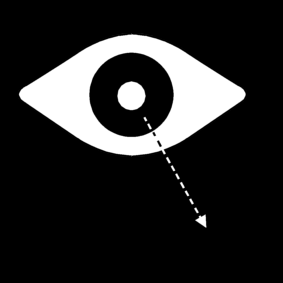
\includegraphics[width=1.5cm]{sclera/zien}\hspace{0.5cm}}
     {
\includegraphics[width=1.5cm]{sclera/bus}\hspace{0.5cm}}
    \begin{xlist}
        \ex \depicto\ (3 of 32):
            \begin{itemize}
                \item \texttt{De hond ziet een bus} (`The dog sees a bus')
                \item \texttt{Een hond zag de bus} (`The dog sees a bus')
                \item \texttt{Honden zien bussen} (`Dogs see buses')
            \end{itemize}
        \ex \emph{Picto2Text}:
            \begin{itemize}
                \item \texttt{De hond ziet een bus} (`The dog sees a bus')
            \end{itemize}
    \end{xlist}
\end{exe}

The output of \emph{Picto2Text} in \cref{ex:conc:dvp1:trans} is already fairly
impressive, since it suggests that somewhere in the training corpus a trigram
occurs which consists (in addition to a third element) of the token \emph{hond}
(`dog') combined with the correctly conjugated form of `barking', i.e.,
\emph{blaft}. When `happy' is added to the start of the \sclera\ string,
however, as in \cref{ex:conc:dvp2:trans}, the result is somewhat different.
Here, in contrast to \depicto, whose output shows the adjective \emph{blij}(+e)
inflecting so as to agree with the gender and/or number of the modified noun
\emph{bus}, \emph{Picto2Text} produces an ungrammatical result: the synonymous
adjective \emph{gelukkig} is not inflected. The inclusion of this extra token
on the input appears to have an obscuring effect on the trigram model, which
now fails to find both the correct third person singular conjugation of the
verb `see' (in this case \emph{ziet}) and a determiner for the count noun
\emph{bus} (although this is technically handled by a separate part of the
system). The reason for this sudden drop in quality is most likely due to the
absence of `happy dog' combinations in the training corpus, as well as to the
general `oddness' of the input string itself, for which a generative approach
can account, but a statistical approach, which by definition favors
conventional language use, cannot.

\begin{exe}
    \ex \label{ex:conc:dvp2:trans} Translating `happy dog see bus' into Dutch: \\\\
     {
\includegraphics[width=1.5cm]{sclera/blij}\hspace{0.5cm}}
     {
\includegraphics[width=1.5cm]{sclera/hond1}\hspace{0.5cm}}
     {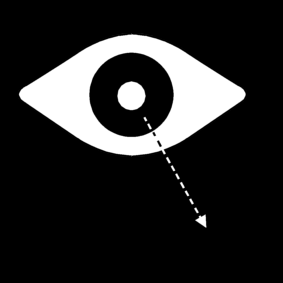
\includegraphics[width=1.5cm]{sclera/zien}\hspace{0.5cm}}
     {
\includegraphics[width=1.5cm]{sclera/bus}\hspace{0.5cm}}
    \begin{xlist}
        \ex \depicto\ (3 of 32):
            \begin{itemize}
                \item \texttt{De blije hond zag de bus} (`The happy dog saw the bus')
                \item \texttt{Blije honden zien de bussen} (`Happy dogs see the buses')
                \item \texttt{Honden zien bussen} (`A happy dog sees the buses')
            \end{itemize}
        \ex \emph{Picto2Text}:
            \begin{itemize}
                \item *\texttt{Gelukkig hond zien bus} (`*Happy dog *see bus')
            \end{itemize}
    \end{xlist}
\end{exe}

A slightly improved situation can be observed in \cref{ex:conc:dvp3:trans}.
Here, the output of \emph{Picto2Text} is grammatical with respect to
determination and conjugation, but presents the present tense form of the verb
`see' as the most likely candidate, in spite of the presence of the temporal
adjunct `yesterday'. (Again, the comparison here is very much biased toward
\depicto, since we have already established that \depicto\ contains a set of
rules to deal precisely with the phenomenon of temporal adjuncts -- that is, provided the encountered temporal adjunct is `yesterday' and nothing else.)

\begin{exe}
    \ex \label{ex:conc:dvp3:trans} Translating `dog see bus yesterday' into Dutch: \\\\
    %  {
\includegraphics[width=1.5cm]{sclera/blij}\hspace{0.5cm}}
     {
\includegraphics[width=1.5cm]{sclera/hond1}\hspace{0.5cm}}
     {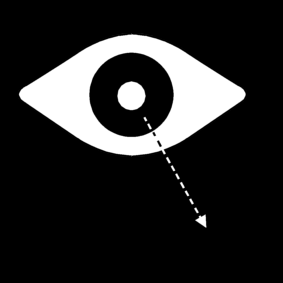
\includegraphics[width=1.5cm]{sclera/zien}\hspace{0.5cm}}
     {
\includegraphics[width=1.5cm]{sclera/bus}\hspace{0.5cm}}
     {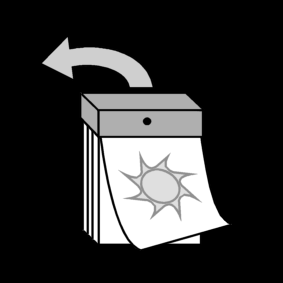
\includegraphics[width=1.5cm]{sclera/gisteren}\hspace{0.5cm}}
    \begin{xlist}
        \ex \depicto\ (3 of 48):
            \begin{itemize}
                \item \texttt{De hond zag de bus gisteren} (`The dog saw the bus yesterday')
                \item \texttt{De honden zagen gisteren de bus} (`The dogs saw the bus yesterday')
                \item \texttt{Een hond zag gisteren de bus} (`A dog saw the bus yesterday')
            \end{itemize}
        \ex \emph{Picto2Text}:
            \begin{itemize}
                \item ?\texttt{de hond ziet een bus gisteren } (`Happy dog
                                ?sees a bus yesterday')
            \end{itemize}
    \end{xlist}
\end{exe}

As we saw in \cref{subs:cs:complex-pictos}, \depicto's analysis module
contains, as it were, specific instructions on how to deal with complex
pictographs. The result is a fair degree of regularity among the various
translation hypotheses produced, as shown in \cref{ex:conc:dvp4:trans} for
`dog+bark'. The output of \emph{Picto2Text}, by contrast, is less easy to
predict -- indeed, surprising: according to the system, the most likely
translation of `dog+bark' is the modified noun phrase `barking dogs', which,
from a strictly communicative perspective, seems like a strange contribution to
make in a conversation (although, of course, that observation is beside the
point in the context of \emph{Picto2Text}'s translation strategy).

\begin{exe}
    \ex \label{ex:conc:dvp4:trans} Translating `dog+bark' into Dutch: \\\\
     {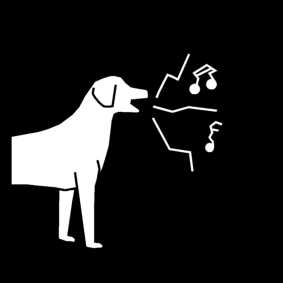
\includegraphics[width=1.5cm]{sclera/hond-blaffen}\hspace{0.5cm}}
    \begin{xlist}
        \ex \depicto\ (3 of 8):
            \begin{itemize}
                \item \texttt{De hond blaft} (`The dog barks')
                \item \texttt{Een hond blafte} (`A dog barked')
                \item \texttt{Honden blaffen} (`Dogs bark')
            \end{itemize}
        \ex \emph{Picto2Text}:
            \begin{itemize}
                \item \texttt{Blaffende honden} (`Barking dogs')
            \end{itemize}
    \end{xlist}
\end{exe}

However, when the first person singular possessive pronoun `my' is added to the
input string, so that we get `my dog+bark', \emph{Picto2Text}'s output, as
shown in \cref{ex:conc:dvp5:trans}, is very different. In this particular case,
the most likely translation according to the language model is the clause
corresponding to `my dog barks'. As far as we are concerned, this is a
perfectly acceptable translation: it is grammatical and its content makes a
communicative contribution which, informationally, seems plausible. It is
interesting to note, moreover, that in this example \emph{Picto2Text} produces
output, whereas \depicto\ does not: possessive pronouns are currently not
covered by the model of \sclera, so the analysis module blocks.

\begin{exe}
    \ex \label{ex:conc:dvp5:trans} Translating `my dog+bark' into Dutch: \\\\
     {\includegraphics[width=1.5cm]{"sclera/spel mijn beurt"}\hspace{0.5cm}}
     {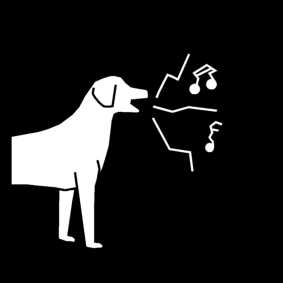
\includegraphics[width=1.5cm]{sclera/hond-blaffen}\hspace{0.5cm}}
    \begin{xlist}
        \ex \depicto\ (0 of 0):
            \begin{itemize}
                \item $\emptyset$
            \end{itemize}
        \ex \emph{Picto2Text}:
            \begin{itemize}
                \item \texttt{Mijn hond blaft} (`My dog barks')
            \end{itemize}
    \end{xlist}
\end{exe}

This illustrates a key point of comparison between the two systems. Whatever
the input, \emph{Picto2Text} will produce output, even if this output is not of
the highest natural linguistic quality. \depicto, by contrast, is picky about
its input, and, even when it accepts it, can fail in any of the two subsequent
stages, depending on how well they are integrated. Yet, when \depicto\
succeeds, its output is consistent (i.e., predictable) and grammatical.
\emph{Picto2tText} is robust, but offers no guarantees about the precision of
its output; \depicto\ is geared toward precision, but is magnificently prone to
failure. Thus, the two systems are each other's inverse -- a point to which we
return in \cref{conc:futurework}.

%-----------------------------------------------------------------------------

\section{Conclusions}

The main objective of the work presented in this thesis is to design and
implement the basic framework for an assistive communication tool that enables
dysphasic users to compose primarily written natural language utterances based
on pictographic symbols. The proposed translation system, \depicto, contrasts
with alternatives (e.g., the \emph{Sanyog}, \emph{PVI}, and \emph{Picto2Text}
systems; see \cref{sec:related-work}) in that its approach is 100\% rule-based.
This goes against the grain of more popular machine translation methodologies,
which tend to favor data-driven or hybrid strategies, but is arguably
appropriate in this particular case, given (a) the lack of resources for
language pairs involving pictographic languages, and (b) the semantically
underspecified and `underquantified' character of pictographic languages in
general. Targeting the \sclera\ symbol set in particular, the \depicto\ system
shows that such languages are amenable to `deep parsing' (i.e., semantic
analysis) in a way that incorporates linguistic intuition (captured as
rules/constraints) to yield consistent and reliable analyses which are
semantically `richer' than the input sequence itself, yet in a way that does
not require structured input from the user (cf. the \emph{Sanyog} system and
its Query-Response input model; \cref{sec:related-work}). The result of deep
parsing (the logical form of the input string) is translated by a set of
bilingual \emph{transfer rules} and used as the basis for target language
generation, which itself is determined by another constraint-based grammar
resource. Because the current version of the system does not filter or rank its
output, the result of generation is a \emph{set} of high-quality translations
of the pictographic input sequence. Insofar as the translation system is
functional, part of this first objective can be said to have been achieved (the
limitations discussed in \cref{subconc:eval:main} notwithstanding). A few
important nuances are returned to in the third paragraph.

On a macro-level, the \depicto\ system requires a total of three resources,
each of which is fairly costly to develop (as one finds out when one develops
them from scratch), in addition to the open-source processor \ace, by means of
which these resources are operationalized (\cref{sub:ace}). A second, more
implicit, objective of the work presented here, therefore, has simply been to
feel out the feasibility of this rule-based approach, especially with respect
to the extensibility of the system to other target languages. To this end, the
criterion is set that the system follow a modular design, the idea being that
the grammar used by the analysis module can be developed independently of other
parts of the grammar so that, in principle, several people can work on it at
once, that is, collaboratively, even if the target language to which they each
individually wish to translate is different. To keep costs down, the
development of the target grammar should ideally not fall within the scope of
the \depicto\ project, but be left to other developers instead; indeed, this is
one of the great advantages of the reusability of \delphin\ grammars. Once the
grammar of \sclera\ reaches an adequate level of coverage (hypothetically, at
least), developers should be able to extend the system to a new language (i.e.,
a different grammar) without requiring too much familiarity with the grammar of
\sclera\ itself, except for its lexicon. In this case, the only remaining work
is situated on the level of the transfer grammar. (As suggested by
\citet{bond2011deep}, much of the work required here can be automated.) In
light of this goal, all parts of the version of \depicto\ presented here have
been designed to adhere to the principle of modularity -- with one important
exception, however, which is that the relation between underspecified and
concrete determiners is currently handled by the target language grammar, whose
type hierarchy contains predicate types specifically for this purpose. If
modularity is to be maintained, therefore, an alternative solution needs to be
devised. This will probably involve the transfer stage, although it may be
possible to relocate it even further `back' in the pipeline, i.e., to the
grammar of \sclera\ itself. \citet{crysmann2012towards} explain that the \ace\
processor allows for so-called \emph{post-parsing rewrite rules}, which are
essentially rewrite rules comparable to those found in the transfer grammar,
except they are included with the parsing grammar and executed, as the term
suggests, as soon as the parser has finished. A definitive solution is deferred
to future work. Of course, it should be borne in mind that, while modularity
certainly improves development costs, particularly if the system garners the
interest of others, these costs remain high in comparison with statistical
machine translation systems. For example, progress on the grammar of \sclera\
will have to be measured in weeks and months rather than days. Whether this is
an adequate trade off for the relatively high translation quality remains to be
seen.

Finally, let us return to the second criterion by which \depicto's design is
guided. Fairly obvious yet essential nonetheless, this criterion requires that
the system stay true to the needs of its target users, who are assumed to be
people with an intellectual (or developmental) disorder that prevents them from
being fully able to produce natural language utterances of an adequately
intelligible or grammatical level. As (part of) a hypothetical alternative
communication tool, the \depicto\ system can be said to meet this criterion
insofar as it is able to accurately translate from pictographic input and thus
provide users with a means of formulating utterances in terms of those
pictographic symbols which are accepted by the system. However, as explained in
\cref{subconc:eval:main}, the current system's analysis module makes a number
of fairly restrictive assumptions about word order, the motivation for which is
explained in more detail above, but boils down to an ad hoc measure to prevent
excessive ambiguity. At present, in the absence of real-life \emph{data}
concerning the use of \sclera\ by the intended user group, it is difficult to
say how great the impact of the SVO word order restriction would be on the
usability of the system by the average user. The question arises whether some
users \emph{are} in fact aware of basic word order patterns, or could be taught
to think in terms of one specific pattern. Of course, even if the answers to
these questions come up positive, it would still imply that another group of
users is excluded from using the system, which is an unfortunate possibility
for a tool whose primary aim is to \emph{improve} inclusion. With regard to
this second criterion, therefore, there is still progress to be made. Closer
interaction with the users themselves, e.g., through user testing or simple
observation, as well as more in-depth research into the syntactic `symptoms' of
dysphasia and other communication disabilities, may serve as an interesting
guideline in this respect.

\section{Future work}
\label{conc:futurework}

In addition to devising near-term solutions to those design decisions that
currently compromise \depicto's criteria of modularity and usability (supra),
future work will concentrate on three main areas.

The first involves the introduction of script-based automation in the modelling
process. The result in the long run should translate to an overall reduction in
the labor-intensitivity of the modelling process, which, of course, goes hand
in hand with a reduction in development time (once an adequate modelling script
has been devised, that is). The most immediate headway can probably be made at
the level of the lexicon of the grammar used by the analysis module, so we will
start there. However, the aim should be to extend script-based automation to as
many parts of the grammar as possible, as well as to the set of transfer rules
used by the next stage in the system. (Modelling the target grammar, by
contrast, is assumed to be the responsibility of a different set of
developers.)

In order to test the idea of modularity, the second area of work involves
switching out the currently used `toy' grammar of Dutch for more extensive (and
mature) grammars of, first, Dutch and, later, other languages, such as English,
German, and Japanese (for which \delphin-based grammars are readily available;
\citet{flickinger2000building,muller2000hpsg,siegel2002efficient}). In
\cref{sec:mini-sclera}, I note that no established \delphin\ grammar of Dutch
is available at the time of writing. This is only partly true.
\citet{fokkens2011metagrammar} includes a grammar of Dutch as part of the
German branch of the CLIMB metagrammar engineering project. Hitherto
unmentioned, the CLIMB project is an offshoot of the Matrix grammar
customization system that builds further on the concept of script-based grammar
generation based on a set of parameters. (The core type hierarchy is the same
as in other Matrix grammars, however.) The CLIMB source code is publicly
available, as are the parameters (which contribute an extensive lexicon)
required for generation of a grammar of Dutch. Unfortunately, despite several
attempts, I was not able to get the CLIMB system to generate a functioning
grammar. This was fairly early on in the development of the \depicto\ system,
however; as I became more familiar with the intricacies of the \delphin\
environment (that is, while I was already working on my own grammar of Dutch),
I came more and more to suspect that this failure was most likely due to error
on my part. The first step in this stage, therefore, will be to revisit the
CLIMB grammar of Dutch, not least because this will require most likely require
minimal modifications to the existing transfer grammar. The next step will
involve the extension of \depicto\ to English. For this we will draw upon the
English Resource Grammar \citep{flickinger2000building} (the flagship grammar
of the \delphin\ project) as well as set up a new transfer grammar.

The third and (by far) most crucial area of future work, however, will concern
the implementation of a method for filtering the output of the target language
generation module down to a single most likely surface realization, which will
bring the behavior of the \depicto\ system in line with that generally expected
of a machine translation system. Currently, there are at least \emph{two}
directions in which we can proceed. As the `likely' in the sentence above might
lead one to expect, both involve some degree of hybridization with
probabilistic strategies, although the approaches themselves do differ.

The first draws further upon the \logon\ MT infrastructure, which, at the
generation end, incorporates a data-driven \emph{realization ranking} component
\citep{velldal2009empirical,velldal2006statistical,bond2011deep}. This
component functions to rank surface realizations (and their underlying
syntactic trees) in order of likeliness as determined by a discriminative
log-linear model trained on an annotated treebank of the target language
\citep{velldal2006statistical}. The highest ranking surface realization forms
the output of translation. This approach is certainly interesting, and should
definitely be explored. Indeed, its developers claim that it represents a great
improvement over `traditional' n-gram approaches (more about which in a moment)
\citep{velldal2009empirical}. Its downsides are that compatible treebanks are
few and far between. There is the \lingo\ Redwoods treebank for English
\citep{Oepen02lingoredwoods}, but equally extensive alternatives for other
languages appear do note appear to exist. At least one \emph{non}-\delphin\
treebank exists for Dutch (see \url{http://nederbooms.ccl.kuleuven.be/eng/}),
but my understanding of treebanking is too limited to conjecture if its
annotations and, most important, syntactic analyses could be transposed to a
\delphin-compatible format. It is currently also unclear whether the \ace\
processor supports realization ranking or whether some additional processor
will be required. The answers to these questions, which will be explored in due
time, will ultimately determine the practicability of the treebanking approach.

The second approach, by contrast, could in principle yield a prototype fairly
quickly. Under this approach, the \depicto\ pipeline is incorporated into
\citet{sevens2015natural}'s \emph{Picto2Text} system (see \cref{sub:picto2text}
and \cref{conc:eval:dep-v-p2t}). The idea is as follows. All input is sent to
\depicto\ first. If the pipeline succeeds, its output is passed to the Viterbi
decoder, the least unlikely string according to which (based on the appropriate
trigram language model) is selected as the output of translation. If the
pipeline fails, the system simply falls back to \emph{Picto2Text}'s original
infrastructure. Alternatively, the two systems are run in parallel and their
output is compared by a second round of Viterbi decoding. Either way, this
approach amplifies the (inverse) strengths of the two systems, while reducing
the effect of their limitations. That is to say, for cases that are easily
covered by a general set of rules, the system as a whole -- `dePicto2Text', if
you will -- is almost guaranteed to produce high-quality output. At the same
time, less easy-to-cover cases will still translate to \emph{something}, the
quality of which, as we see in \cref{conc:eval:dep-v-p2t}, \emph{is} more
variable but can also be just as high as that achieved by \depicto. Thus, the
average precision of the modified \emph{Picto2Text} increases, while the
robustness of the original system stays exactly the same. An added bonus to
this approach is that \depicto\ gets to piggyback on (and, if desired,
contribute to) \emph{Picto2Text}'s user interface. Besides the convenience of
freeing up initial development time, this could ultimately translate to more
progress on the interface in less time. Given all its advantages, the second
approach is the most interesting. Of course, is is \emph{only} a proposal. For
now, therefore, we keep our options open.
